\documentclass{article}
\usepackage{cmap}
\usepackage[utf8]{inputenc}
\usepackage[english,ukrainian]{babel}
\usepackage{graphicx}
\usepackage{geometry}
\usepackage{listings}
\usepackage{float}
\usepackage{amsmath}
\geometry{
	a4paper,
	left=20mm,
	right=20mm,
	top=15mm,
	bottom=15mm,
}
\lstset{
	language=c,
	tabsize=4,
	keepspaces,
	showstringspaces=false,
}
\graphicspath{ {./pictures} }
\setlength{\parindent}{4em}

\newcommand\subject{Основи електроніки}
\newcommand\lecturer{професор кафедри ПЗ \\ Фечан А.В.}
\newcommand\teacher{доцент кафедри ПЗ \\ Коцун В.І.}
\newcommand\mygroup{ПЗ-22}
\newcommand\lab{4}
\newcommand\theme{Дослідження напівпровідникових випрямлячів}
\newcommand\purpose{Дослідження роботи випрямлячів змінної напруги на прикладі схем: однопівперіодної, двопівперіодної із середньою точкою, однофазної мостової. Ознайомитися із принципом дії і основними характеристиками фільтрів, що
	згладжують}

\begin{document}
\begin{normalsize}
	\begin{titlepage}
		\thispagestyle{empty}
		\begin{center}
			\textbf{МІНІСТЕРСТВО ОСВІТИ І НАУКИ УКРАЇНИ\\
				НАЦІОНАЛЬНИЙ УНІВЕРСИТЕТ "ЛЬВІВСЬКА ПОЛІТЕХНІКА"}
		\end{center}
		\begin{flushright}
			\textbf{ІКНІ}\\
			Кафедра \textbf{ПЗ}
		\end{flushright}
		\vspace{200pt}
		\begin{center}
			\textbf{ЗВІТ}\\
			\vspace{10pt}
			до лабораторної роботи № \lab\\
			\textbf{на тему}: “\textit{\theme}”\\
			\textbf{з дисципліни}: “\subject”
		\end{center}
		\vspace{112pt}
		\begin{flushright}
			
			\textbf{Лектор}:\\
			\lecturer\\
			\vspace{28pt}
			\textbf{Виконав}:\\
			
			студент групи \mygroup\\
			Коваленко Д.М.\\
			\vspace{28pt}
			\textbf{Прийняв}:\\
			
			\teacher\\
			
			\vspace{28pt}
			«\rule{1cm}{0.15mm}» \rule{1.5cm}{0.15mm} 2023 р.\\
			$\sum$ = \rule{1cm}{0.15mm}……………\\
			
		\end{flushright}
		\vspace{\fill}
		\begin{center}
			\textbf{Львів — 2023}
		\end{center}
	\end{titlepage}
		
	\begin{description}
		\item[Тема.] \theme.
		\item[Мета.] \purpose.
	\end{description}

	\section*{Теоретичні відомості}
	
	Для перетворення змінної напруги в постійну напругу застосовують випрямні
	пристрої. У випрямний пристрій звичайно входять трансформатор, один або
	кілька діодів, фільтр, що згладжує, електронний стабілізатор постійної напруги.
	Залежно від умов роботи окремі елементи випрямного пристрою можуть бути
	відсутніми.
	
	Вибір тієї або іншої схеми джерела напруги вторинного живлення обумовле-
	ний параметрами живильної мережі, вимогами до вихідних електричних парамет-
	рів, конструктивним особливостями пристрою, температурним діапазоном роботи,
	терміном служби, гарантованою надійністю і переліком дозволених до застосу-
	вання елементів.
	
	більшості випадків для живлення вимірювальних приладів використовуєть-
	ся однофазна мережа, з діючим значенням напруги 220 В, 50 Гц.
	Схема однопівперіодного випрямляча наведена на рис.1,а.
	Для спрощення аналізу будемо вважати діод ідеальним, тобто будемо думати,
	що його опір в прямому напрямку дорівнює нулю, a y зворотному - нескінченнос-
	ті. Тоді протягом першого півперіоду вхідної напруги, коли на аноді діода VD бу-
	де позитивний щодо катода потенціал, діод буде відкритий.
	
		\section*{Індивідуальне завдання}
	Дослідити вольт-амперні характеристики діода, стабілітрона (діода Зенера) та світлодіода (LED).
	
	Складіть схему, що дозволяє досліджувати вольт-амперні характеристики різних діодів (1N4148 –звичайний діод; 1N4733 –стабілітрон; greenLED–світлодіод)
	
	Використовуючи осцилограми напруги на діодах як аналоги струму через ці діоди (I = U/R, де R = 1 Ohm), визначіть на збільшеній осцилограмі значення порогової напруги (U0); внутрішнього опору Rвн діода при апроксимації його математичною моделлю виду Uд = U0 + Rвн·Iд. Порівняйте отримані залежності Uд(Iд) для досліджуваних діодів.
	
	Складіть схему що моделює однопівперіодний випрямляч із ємнісним фільтром.
	
	Змінюючи опір навантаження Rch від 10 kOhm до 500 Ohm, при ємності фільтра 
 Сfiltr =  100  $\mu F$,  зафіксувати  показання  вольтметрів,  що  вимірюють постійну Ucon і змінну Ualt складові вихідної напруги. Дані звести в таблицю.
 
	Побудуйте залежності Kп(Ich) і Ucon(Ich). Визначіть внутрішній опір випрямляча
	 Змалювати осцилограми U~(t) і Uch(t) при Rch= 10 kOhm і Rch= 500 Ohm.
	Повторіть п.п. 5-6 при Сfiltr= 100 pF. Визначіть вплив величини Сfiltr на якість випрямленої напруги.
	
	Складіть схему, що моделює двопівперіодний випрямляч із ємнісним фільтром.
	
	Повторіть п.п 5-6 для цієї схеми.
	
	
	\section*{Хід виконання}
	1. Склав схему, яка дозволяє досліджувати вольт-амперні характеристики різних діодів (1N4148 – звичайний діод; 1N4733 – стабілітрон; green\_LED – світлодіод).
	
	\begin{figure}[H]
		\begin{minipage}[t]{0.55\textwidth}
			\centering
			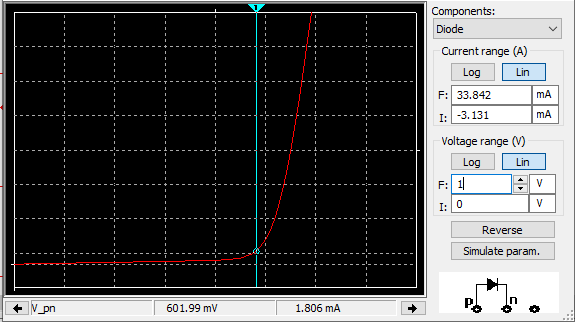
\includegraphics[width=\textwidth]{11}
		\end{minipage}
		\hfill
		\begin{minipage}[t]{0.35\textwidth}
			\centering
			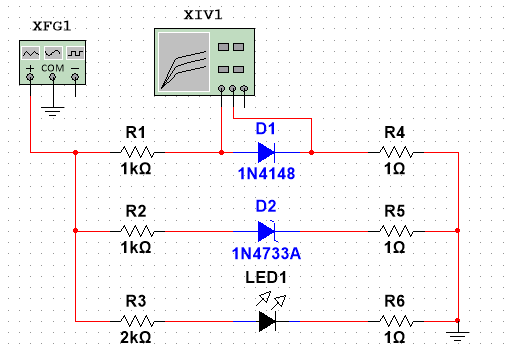
\includegraphics[width=\textwidth]{12}
		\end{minipage}
		\caption{Вольт-амперна характеристика звичайного діода.}
	\end{figure}
	
	\begin{figure}[H]
		\begin{minipage}[t]{0.55\textwidth}
			\centering
			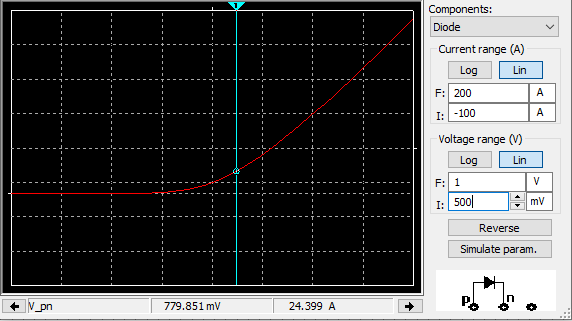
\includegraphics[width=\textwidth]{21}
		\end{minipage}
		\hfill
		\begin{minipage}[t]{0.35\textwidth}
			\centering
			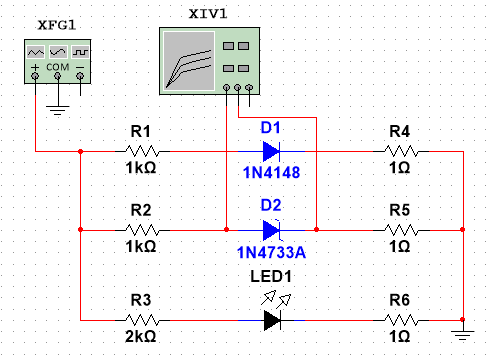
\includegraphics[width=\textwidth]{22}
		\end{minipage}
		\caption{Вольт-амперна характеристика діода Зенера.}
	\end{figure}

	\begin{figure}[H]
		\begin{minipage}[t]{0.55\textwidth}
			\centering
			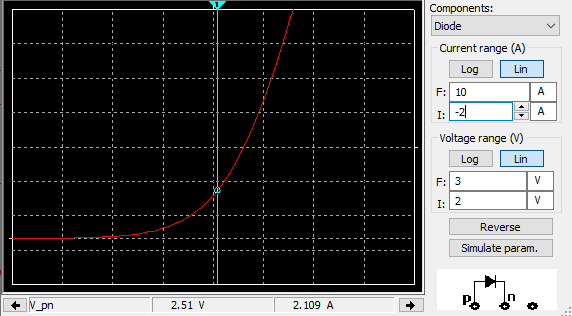
\includegraphics[width=\textwidth]{31}
		\end{minipage}
		\hfill
		\begin{minipage}[t]{0.35\textwidth}
			\centering
			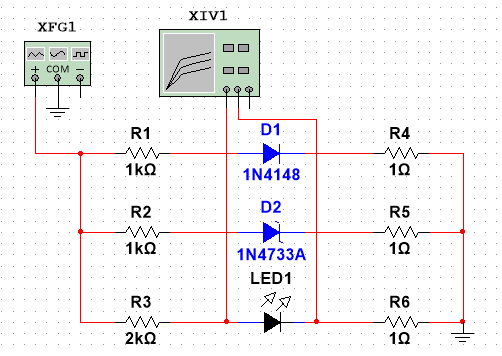
\includegraphics[width=\textwidth]{32}
		\end{minipage}
		\caption{Вольт-амперна характеристика світлодіода.}
	\end{figure}
	
	2. Використовуючи вольт-амперну характеристику діодів, знайшов значення порогової напруги:
	
	\begin{table}[H]
		\centering
		\renewcommand*\arraystretch{1.3}
		\begin{tabular}{|p{0.25\linewidth}|p{0.1\linewidth}|}
			\hline
			\textbf{Звичайний діод} & 0.675 В\\
			\hline
			\textbf{Діод Зенера} & 0.780 В\\
			\hline
			\textbf{Світлодіод} & 2.51 В\\
			\hline
		\end{tabular}
	\end{table}
	
	3. Змінюючи опір навантаження $R_{ch}$ від 10 $kOhm$ до 500 $Ohm$, при ємності фільтра $C_{filtr}$ = 100 $\mu F$, зафіксував показання вольтметрів, що вимірюють постійну $U_{con}$ і змінну $U_{alt}$ складові вихідної напруги.
	
	\begin{table}[H]
		\centering
		\renewcommand*\arraystretch{1.3}
		\begin{tabular}{|p{0.15\linewidth}|p{0.08\linewidth}|p{0.08\linewidth}|p{0.08\linewidth}|p{0.08\linewidth}|p{0.08\linewidth}|}
			\hline
			$R_{ch}$, $kOhm$& 10 & 5 & 2 & 1 & 0.5\\
			\hline
			$I_{ch}$, $mA$& 1.6 & 3.2 & 7.8 & 15.1 & 28.5\\
			\hline
			$U_{con}$, $V$& 16.1 & 16 & 15.7 & 15.1 & 14.2\\
			\hline
			$U_{alt}$, $V$& 0.07 & 0.15 & 0.35 & 0.67 &1.2\\
			\hline
			$K_\text{п}=U_{con}/U_{m}$& 162.6 & 75.4 & 31.7 & 15.9 & 8.4\\
			\hline
		\end{tabular}
		\caption{$C_{filtr}$ = 100 $\mu F$}
	\end{table}
	
		\begin{figure}[H]
			\centering
			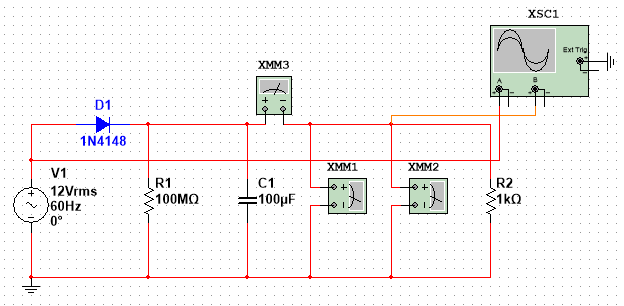
\includegraphics[width=\textwidth]{2}
			\caption{Схема}
	\end{figure}

	\begin{figure}[H]
		\begin{minipage}[t]{0.48\textwidth}
			\centering
			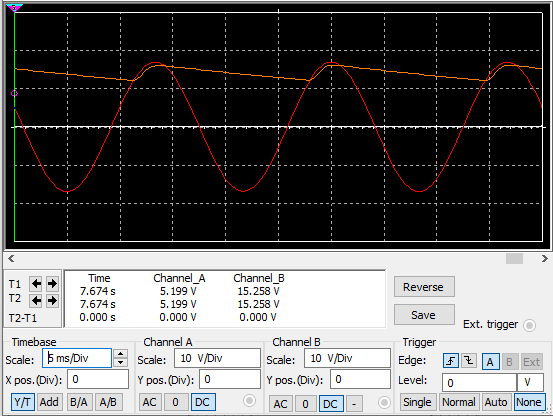
\includegraphics[width=\textwidth]{500}
			\caption{$R_{ch}=500\text{ Ohm}$, $C=100\mu F$}
		\end{minipage}
		\hfill
		\begin{minipage}[t]{0.48\textwidth}
			\centering
			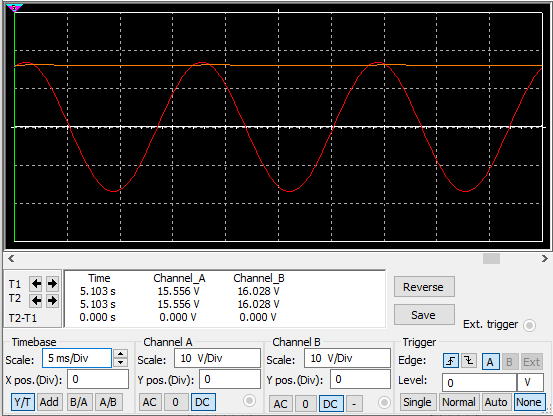
\includegraphics[width=\textwidth]{10k}
			\caption{$R_{ch}=10k\text{ Ohm}$, $C=100\mu F$}
		\end{minipage}
	\end{figure}
	
	\begin{figure}[H]
		\begin{minipage}[t]{0.48\textwidth}
			\centering
			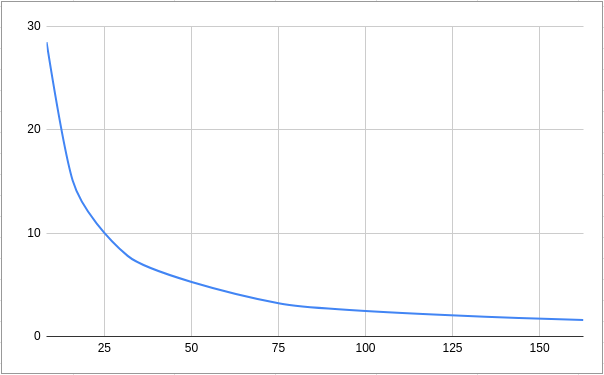
\includegraphics[width=\textwidth]{g1}
			\caption{$K_\text{п}/I_{ch}$}
		\end{minipage}
		\hfill
		\begin{minipage}[t]{0.48\textwidth}
			\centering
			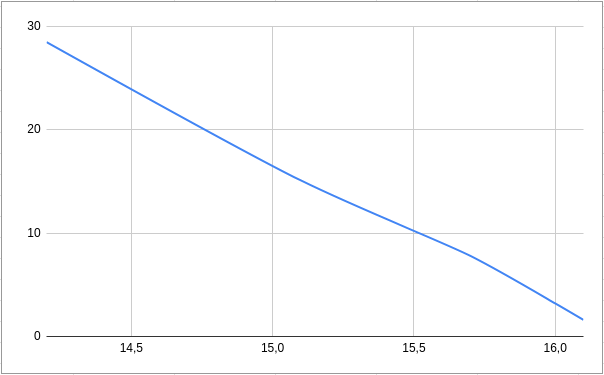
\includegraphics[width=\textwidth]{g2}
			\caption{$U_{con}/I_{ch}$}
		\end{minipage}
	\end{figure}

	Внутрішній опір	випрямляча:
	\begin{gather}
		R_{вн}=\frac{\delta U_{con}}{\delta U_{ch}}=\frac{0.5}{10}=0.05 \text { Ohm}.\nonumber
	\end{gather}

	4. Змінюючи опір навантаження $R_{ch}$ від 10 $kOhm$ до 500 $Ohm$, при ємності фільтра $C_{filtr}$ = 100 $pF$, зафіксував показання вольтметрів, що вимірюють постійну $U_{con}$ і змінну $U_{alt}$ складові вихідної напруги.

	\begin{table}[H]
		\centering
		\renewcommand*\arraystretch{1.3}
		\begin{tabular}{|p{0.15\linewidth}|p{0.08\linewidth}|p{0.08\linewidth}|p{0.08\linewidth}|p{0.08\linewidth}|p{0.08\linewidth}|}
			\hline
			$R_{ch}$, $kOhm$& 10 & 5 & 2 & 1 & 0.5\\
			\hline
			$I_{ch}$, $mA$& 0.5 & 1 & 2.5 & 5 & 10.1\\
			\hline
			$U_{con}$, $V$& 5.1 & 5 & 5 & 5 & 5\\
			\hline
			$U_{alt}$, $V$& 6.3 & 6.2 & 6.2 & 6.2 &6.2\\
			\hline
			$K_\text{п}=U_{con}/U_{m}$& 0.57 & 0.57 & 0.57 & 0.57 & 0.57\\
			\hline
		\end{tabular}
		\caption{$C_{filtr}$ = 100 $pF$}
	\end{table}
	
	6.  Склав схему, яка моделює двопівперіодний ‘випрямляч із ємнісним фільтром.
	
			\begin{figure}[H]
		\centering
		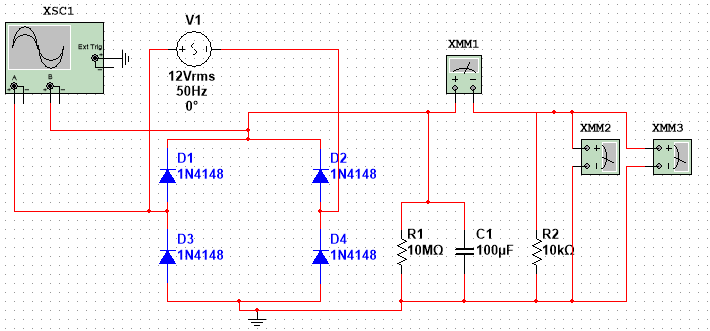
\includegraphics[width=\textwidth]{s3}
		\caption{Схема}
	\end{figure}
	
	
	7.  Змінюючи опір навантаження $R_{ch}$ від $10\text{ kOhm}$ до $500\text{ Ohm}$, зафіксував показання вольтметрів, що вимірюють постійну $U_{con}$і змінну $U_{alt}$ складові вихідної напруги.
	
	\begin{table}[H]
		\centering
		\renewcommand*\arraystretch{1.3}
		\begin{tabular}{|p{0.15\linewidth}|p{0.08\linewidth}|p{0.08\linewidth}|p{0.08\linewidth}|p{0.08\linewidth}|p{0.08\linewidth}|}
			\hline
			$R_{ch}$, $kOhm$& 10 & 5 & 2 & 1 & 0.5\\
			\hline
			$I_{ch}$, $mA$& 1.5 &3 & 7.6 & 14.8 & 29 \\
			\hline
			$U_{con}$, $V$& 15.5 & 15.4 & 15.2 & 14.8 & 14.3\\
			\hline
			$U_{alt}$, $V$& 0.04 & 0.08 & 0.18 & 0.36 & 0.67\\
			\hline
			$K_\text{п}=U_{con}/U_{m}$& 274 & 136.1 & 59 & 29 & 15.9\\
			\hline
		\end{tabular}
				\caption{$C_{filtr}$ = 100 $\mu F$}
	\end{table}
	
	\begin{figure}[H]
		\begin{minipage}[t]{0.48\textwidth}
			\centering
			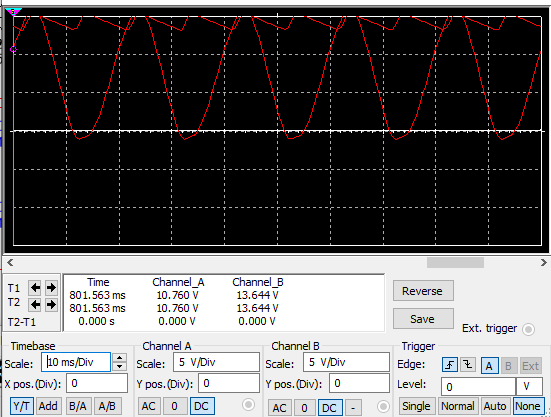
\includegraphics[width=\textwidth]{41}
			\caption{Графік роботи двопівперіодного випрямляча змінної напруги з конденсатором}
		\end{minipage}
		\hfill
		\begin{minipage}[t]{0.48\textwidth}
			\centering
			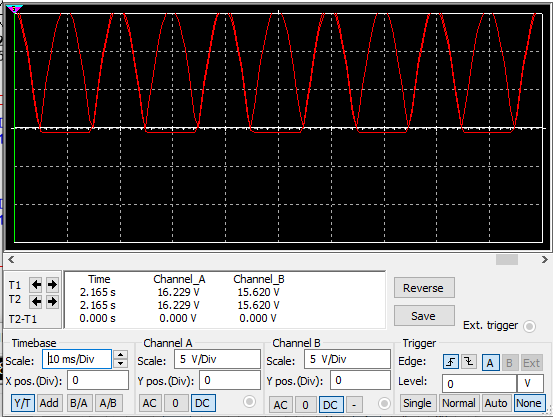
\includegraphics[width=\textwidth]{43}
			\caption{Графік роботи двопівперіодного випрямляча змінної напруги без конденсатора}
		\end{minipage}
	\end{figure}
	
		\begin{figure}[H]
		\begin{minipage}[t]{0.48\textwidth}
			\centering
			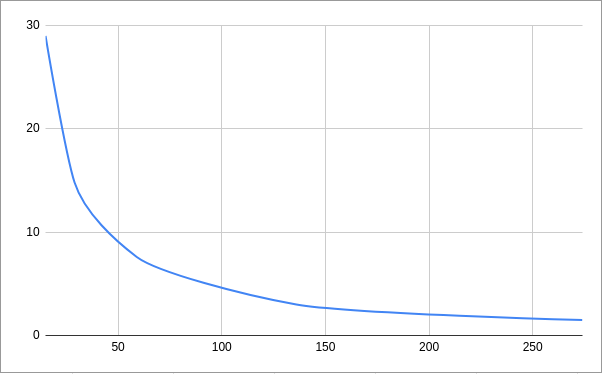
\includegraphics[width=\textwidth]{g4}
			\caption{$K_\text{п}/I_{ch}$}
		\end{minipage}
		\hfill
		\begin{minipage}[t]{0.48\textwidth}
			\centering
			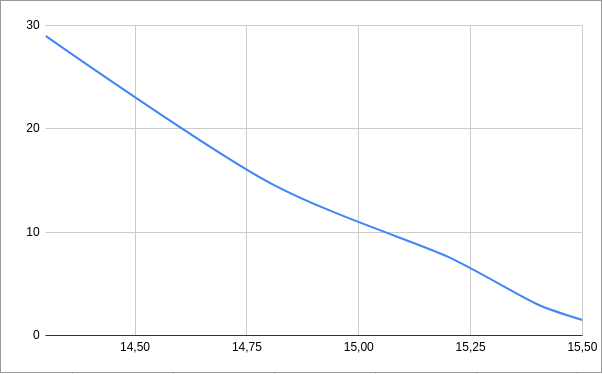
\includegraphics[width=\textwidth]{g3}
			\caption{$U_{con}/I_{ch}$}
		\end{minipage}
	\end{figure}
	
	\section*{Висновки}
	Під час виконання лабораторної роботи я дослідив роботи випрямлячів змінної напруги на прикладі схем: однопівперіодної, двопівперіодної із середньою точкою, однофазної мостової. Ознайомився із принципом дії і основними характеристиками фільтрів, що згладжують.
	    
\end{normalsize}
\end{document}
